% Preamble

\documentclass[11pt]{article}

% Packages
\usepackage{amsmath}
\usepackage{mathtools}
\usepackage{ragged2e}
\usepackage [utf8]{inputenc}
\usepackage{blindtext}
\usepackage{wrapfig}
\usepackage{xcolor}
\usepackage {polski}
\usepackage{multicol}
\usepackage[a4paper, total={5.7in, 8in}]{geometry}
\usepackage{graphicx}
\usepackage{amstex}
\usepackage{csvsimple}
\usepackage{changepage}
\usepackage{enumitem}
\usepackage[english]{babel}
\usepackage{biblatex}
\usepackage{caption}
\usepackage{indentfirst}
\usepackage{epstopdf-base}
\usepackage{textcomp}
\usepackage{wasysym}

% Document
\begin{document}
%    Nagłówek
    \begin{flushleft}
        Maciej Pierzchała 282 934 \hfill Data wykonania ćwiczenia:\\
        Filip Kubecki 272 655 \hfill 26 listopada 2024r\\
        Grupa: Wtorek 10:35 \\
    \end{flushleft}
    \begin{center}
        \Large\textbf{Laboratorium 7}\\
        \textbf{Charakteryzacja czujnika spektrofotometrycznego}
    \end{center}
    \hfill
    \vspace{2cm}
%    Treść
    \section{Spis przyrządów}
    \par{
        Do wykonania ćwiczenia wykorzystano:
        \begin{itemize}
            \setlength\itemsep{0em}
            \item[-] Zasilacz labolatoryjny
            \item[-] Źródła światła: świetlówki(CFL), żarówki, LED i halogeny
            \item[-] Oranż metylowy - $C_{14}H_{14}N_{3}NAO_{3}S$
            \item[-] Spektrofotometr
            \item[-] Pipeta
            \item[-] Pomocnicze szkło labolatoryjne: zlewki, butelki
        \end{itemize}
    }
    \section{Przebieg i cele doświadczenia}
    \par\noindent Celami ćwiczenia było porównianie charakterystyk spektroskopowych różnych typów źródeł światła oraz wyciągnięcie
    wniosków na temat tego jakie ze źródeł najbardziej odpowiada ludzkiemu oku. Należało również zbadać natężenie światła przepuszczanego
    przez roztwory oranżu metylowego o różnych stężeniach i określić poziom ich absorbcji. Na podstawie tych danych należało wyznaczyć krzywą
    kalibracji i wyznaczyć stężenie próbki o nieznanym stężeniu.
\newpage
    \section{Obliczenia i analiza wyników}
    \subsection{Analiza porównawcza różnych źródeł światła}
%    \par\textbf{Na poniższym wykresie przedstawiono porównanie spektrum każdego źródła światła:} \\
    \noindent\makebox[\textwidth]{
        \includegraphics[scale = 0.6]{/home/bork/IdeaProjects/LatexProjects/src/PodstawyTechnikiSensorowej/Lab7/Img/plot1}}
    \justifying\indent Na podstawie wykresu można odrazu wysunąć dwa wnioski: świetlówka posiada spetkrum składające się z
    ostrych pików pewnych wąskich zakresów częstotliwości oraz spektrum lampy żarowej posiada bardzo płaskie spektrum
    w którym nie ma pików żadnej długości fali. W źródle żarowym jedynie widać większą amplitudę dla części czerwonego światła
    co może przekładać się na nasz ostateczny odbiór światła lamp żarowych jako pomarańczowo czerwone.\\
    \indent W przypadku źródla LED możemy wyróżnić trzy znaczące piki występujące w rejonach długości fali przypisanym
    kolorowi czerwonemu, zielonemu i niebieskiego. Wynika to z budowy tego typu źródeł światła które posiada przeważnie
    konfigurację diód LED o tych specyficznych kolorach. Te kolory odpowiadają długościom fal które odbierają
    czopki znajdujące się w naszych oczach. Można również zauważyć że pik w zakresie koloru zielonego jest mniejszy
    niż dla niebieskiego oraz czerwonego co wynika z tego że ludzkie oczy posiadają dwa razy więcej czopków odbierających
    kolor zielony. Wymagają one więc niższej stymulacji.\\
    \indent Ostatnie źródło czyli lampa halogenowa posiada spekrum podobne do tego lamy LED lecz posiadające dwie
    wyróżniające cechy. Po pierwsze pik w rejonie niebieskim ma o wiele niższą amplitudę a po drugie zakres koloru czerwonego
    jest o wiele szerszy i przechodzi płynnie w podczerwień.\\
    \indent Zastanawiając się jaki typ źródła światła z badanych posiada najlepsze parametry dla oczu należy zdefiniować
    samo pojęcie światłą dobrego dla oka. Jeżeli jest to światło które najmniej męczy oczy będą to źródła posiadające bardzo
    szerokie zakresy światła czerwonego oraz małe i niskie zakresy światła niebieskiego i zielonego. Najlepszymi kandydatami
    będą tutaj światło żarówki i lampy halogenowej.\\
    \indent Jeżeli chcemy otrzymać światło które najlepiej odwzorowuje kolory rzeczywiste (te występujące przy świetle naturalnym)
    lepszym wyborem będzie światło lampy LED. Przez posiadanie wszystkich kolorów odbieranych przez oczy w odpowiednich proporcjach
    pozwala ono widzieć nam materiały na takie jakie są rzeczywiste podczas gdy światło źródeł z przeważaniem koloru czerwonego lub
    niebieskiego może dawać złudne wrażenie "pomarańczowości" kolorów.

%    \centering\textbf{Na poniższym wykresie porównano spektrum źródeł światła typu LED:} \\
    \noindent\makebox[\textwidth]{
        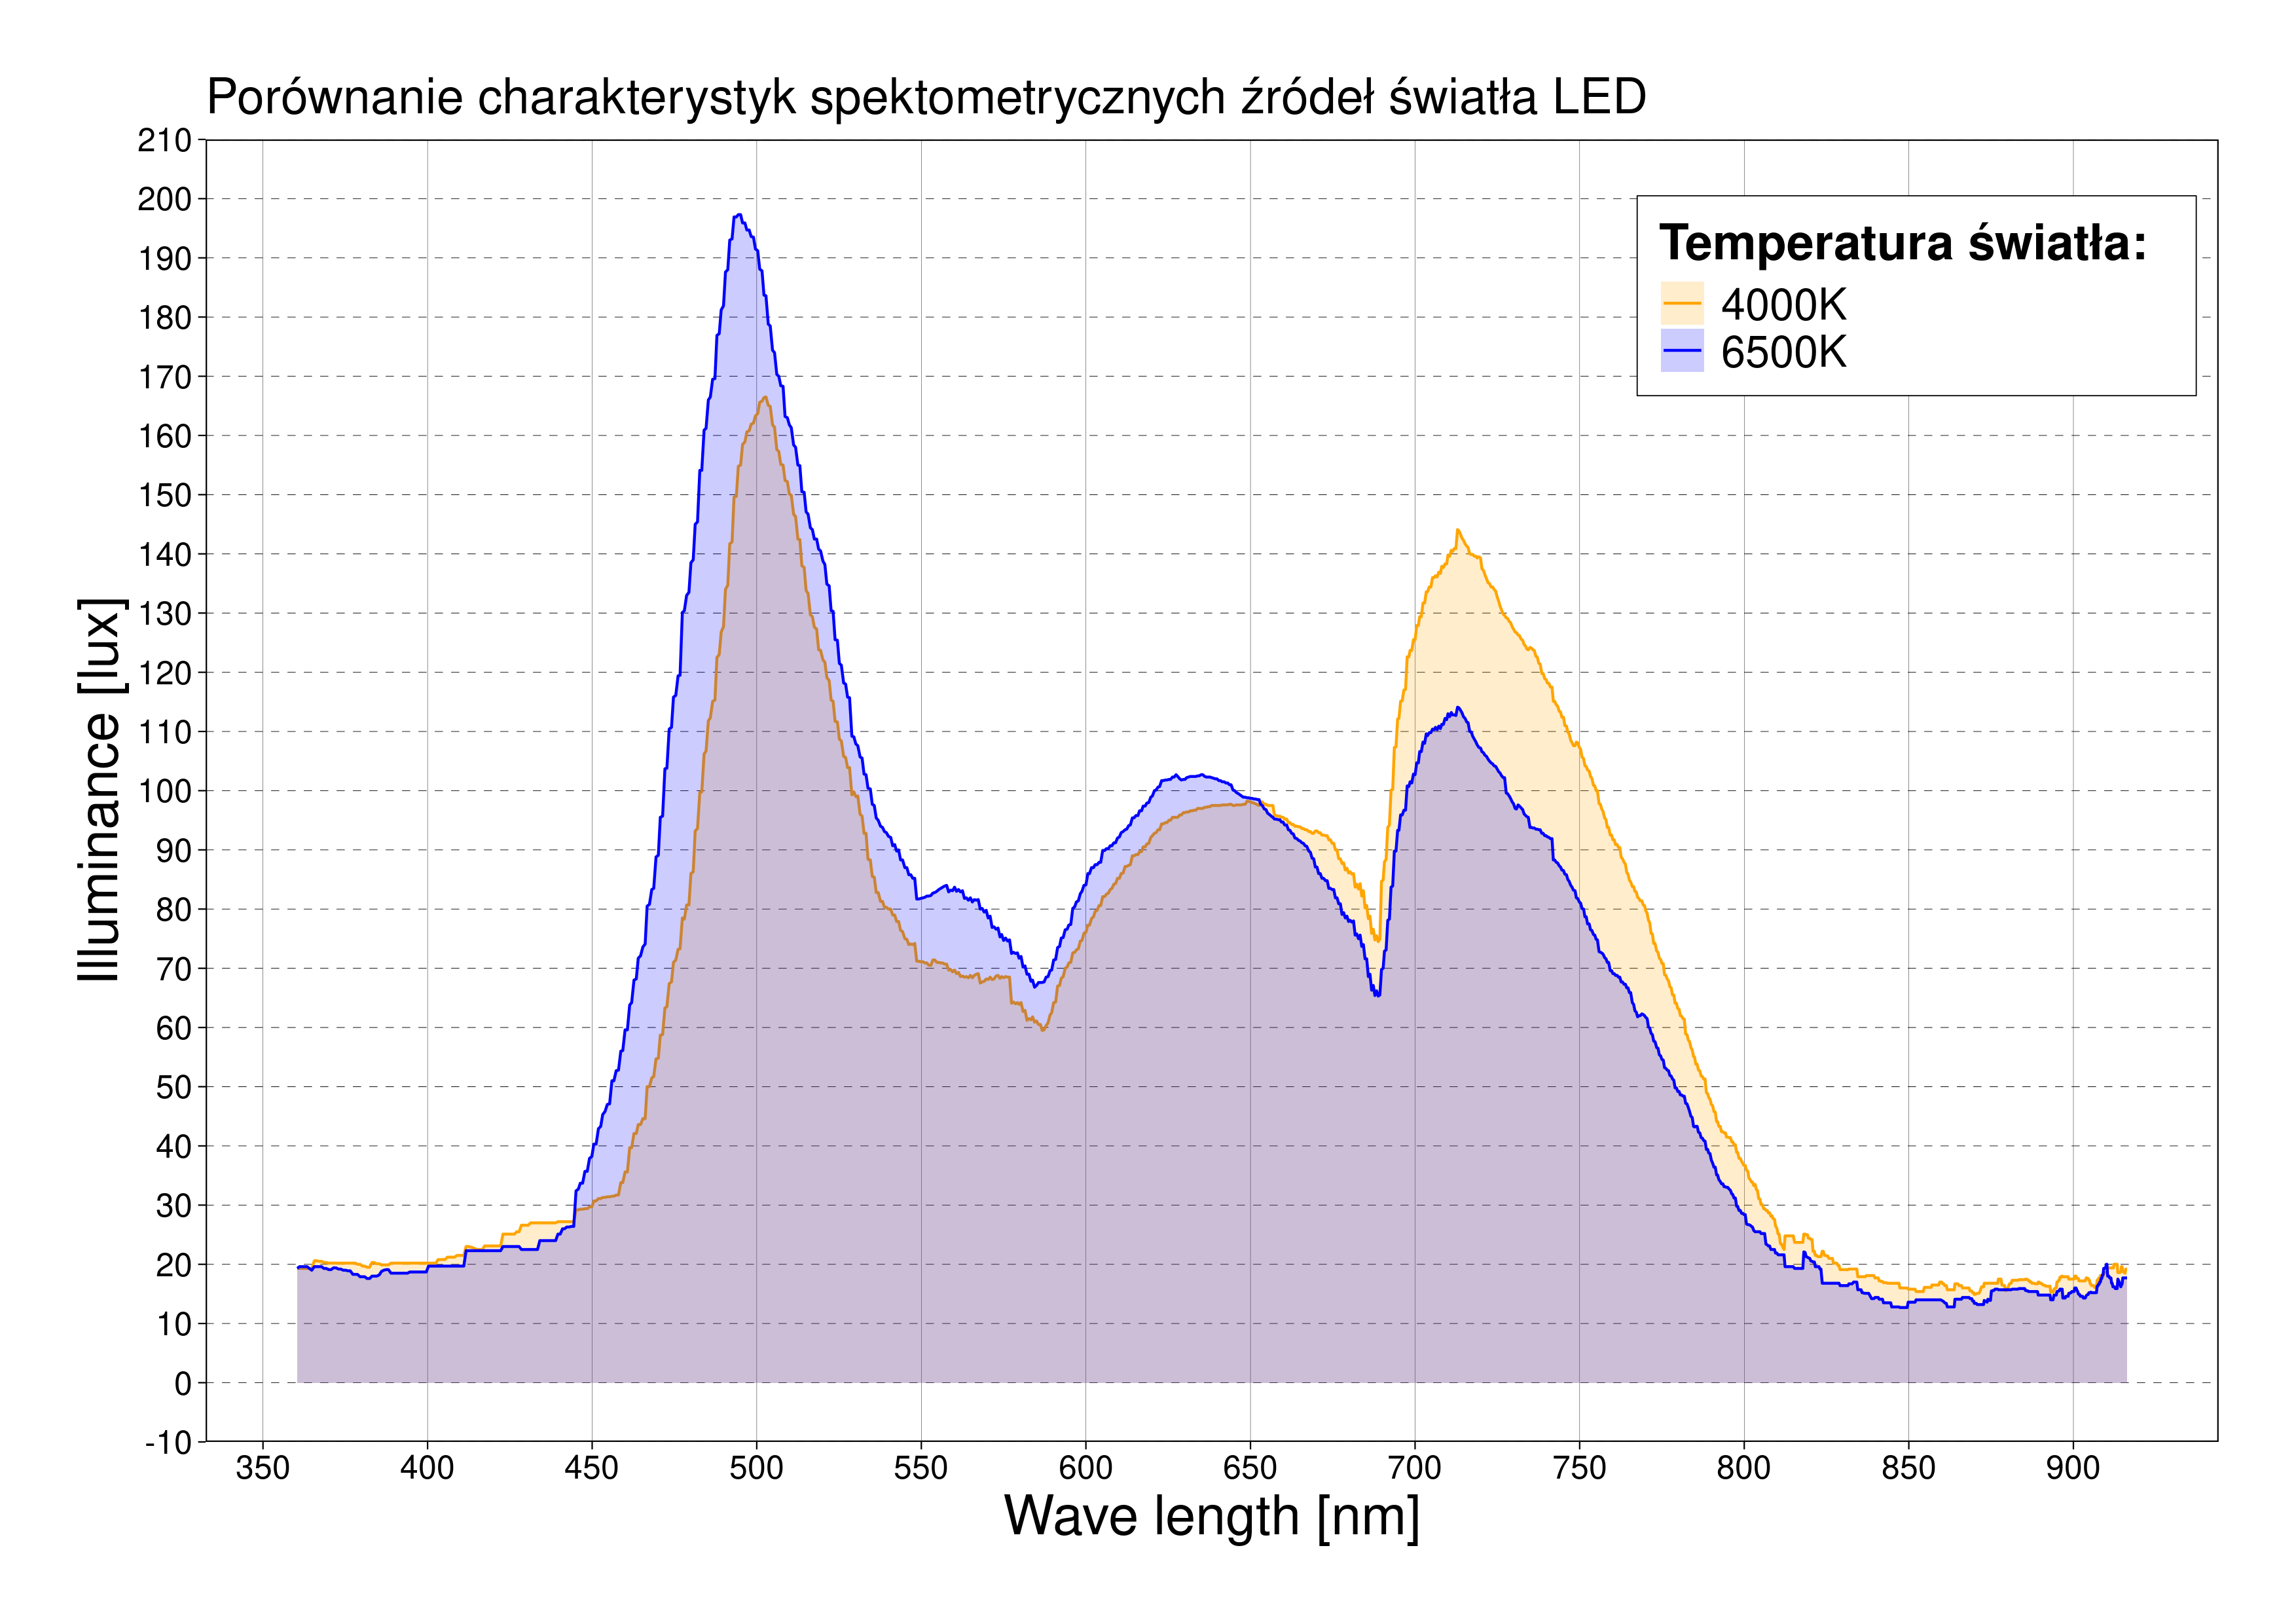
\includegraphics[scale = 0.57]{/home/bork/IdeaProjects/LatexProjects/src/PodstawyTechnikiSensorowej/Lab7/Img/plot3}}
    \indent Na powyższym wykresie możemy zaobserwować w jaki sposób producenci uzyskują różną temperaturę światła
    w przypadku lamp LED. Oba źródła światła posiadają charakterystyki o bardzo podobnym kształcie jednak różnią się amplitudami
    w nitkórych zakresach. Gdy popatrzymy na światło o temparaturze $4000[K]$ możemy zauważyć wyższy pik w zakresie barwy czerwonej
    oraz niższy pik w zakresie koloru niebieskiego. Pik koloru zielonego w obu przypadkach różni sie na tyle nieznacząco że można przyjąć
    że wyglądają one identycznie. Ciepło światła możemy więc regulować proporcją światła emitowanego przez diody czerwone oraz przez diody
    niebieskie. W przypadku lamp LED jest to bardzo proste gdyż wymaga to regulacji natężenia poprzez zmianę rezystancji rezystorów zasilajacych
    diodę LED. Tworząc układ posiadający regulowany poziom zasilania dla kolejnych kolorów diód LED możemy stworzyć lampę która potrafi wyemitować
    dowolne światło. Lampy takie głównie spotykają swoje zastosowanie w kinematografi oraz fotografi lecz stają się coraz popólarniejsze w
    zastosowaniach na rynku domowym.

%    \centering\textbf{Na poniższym wykresie porównano spektrum dwóch źródeł światła typu CFL:} \\
    \noindent\makebox[\textwidth]{
        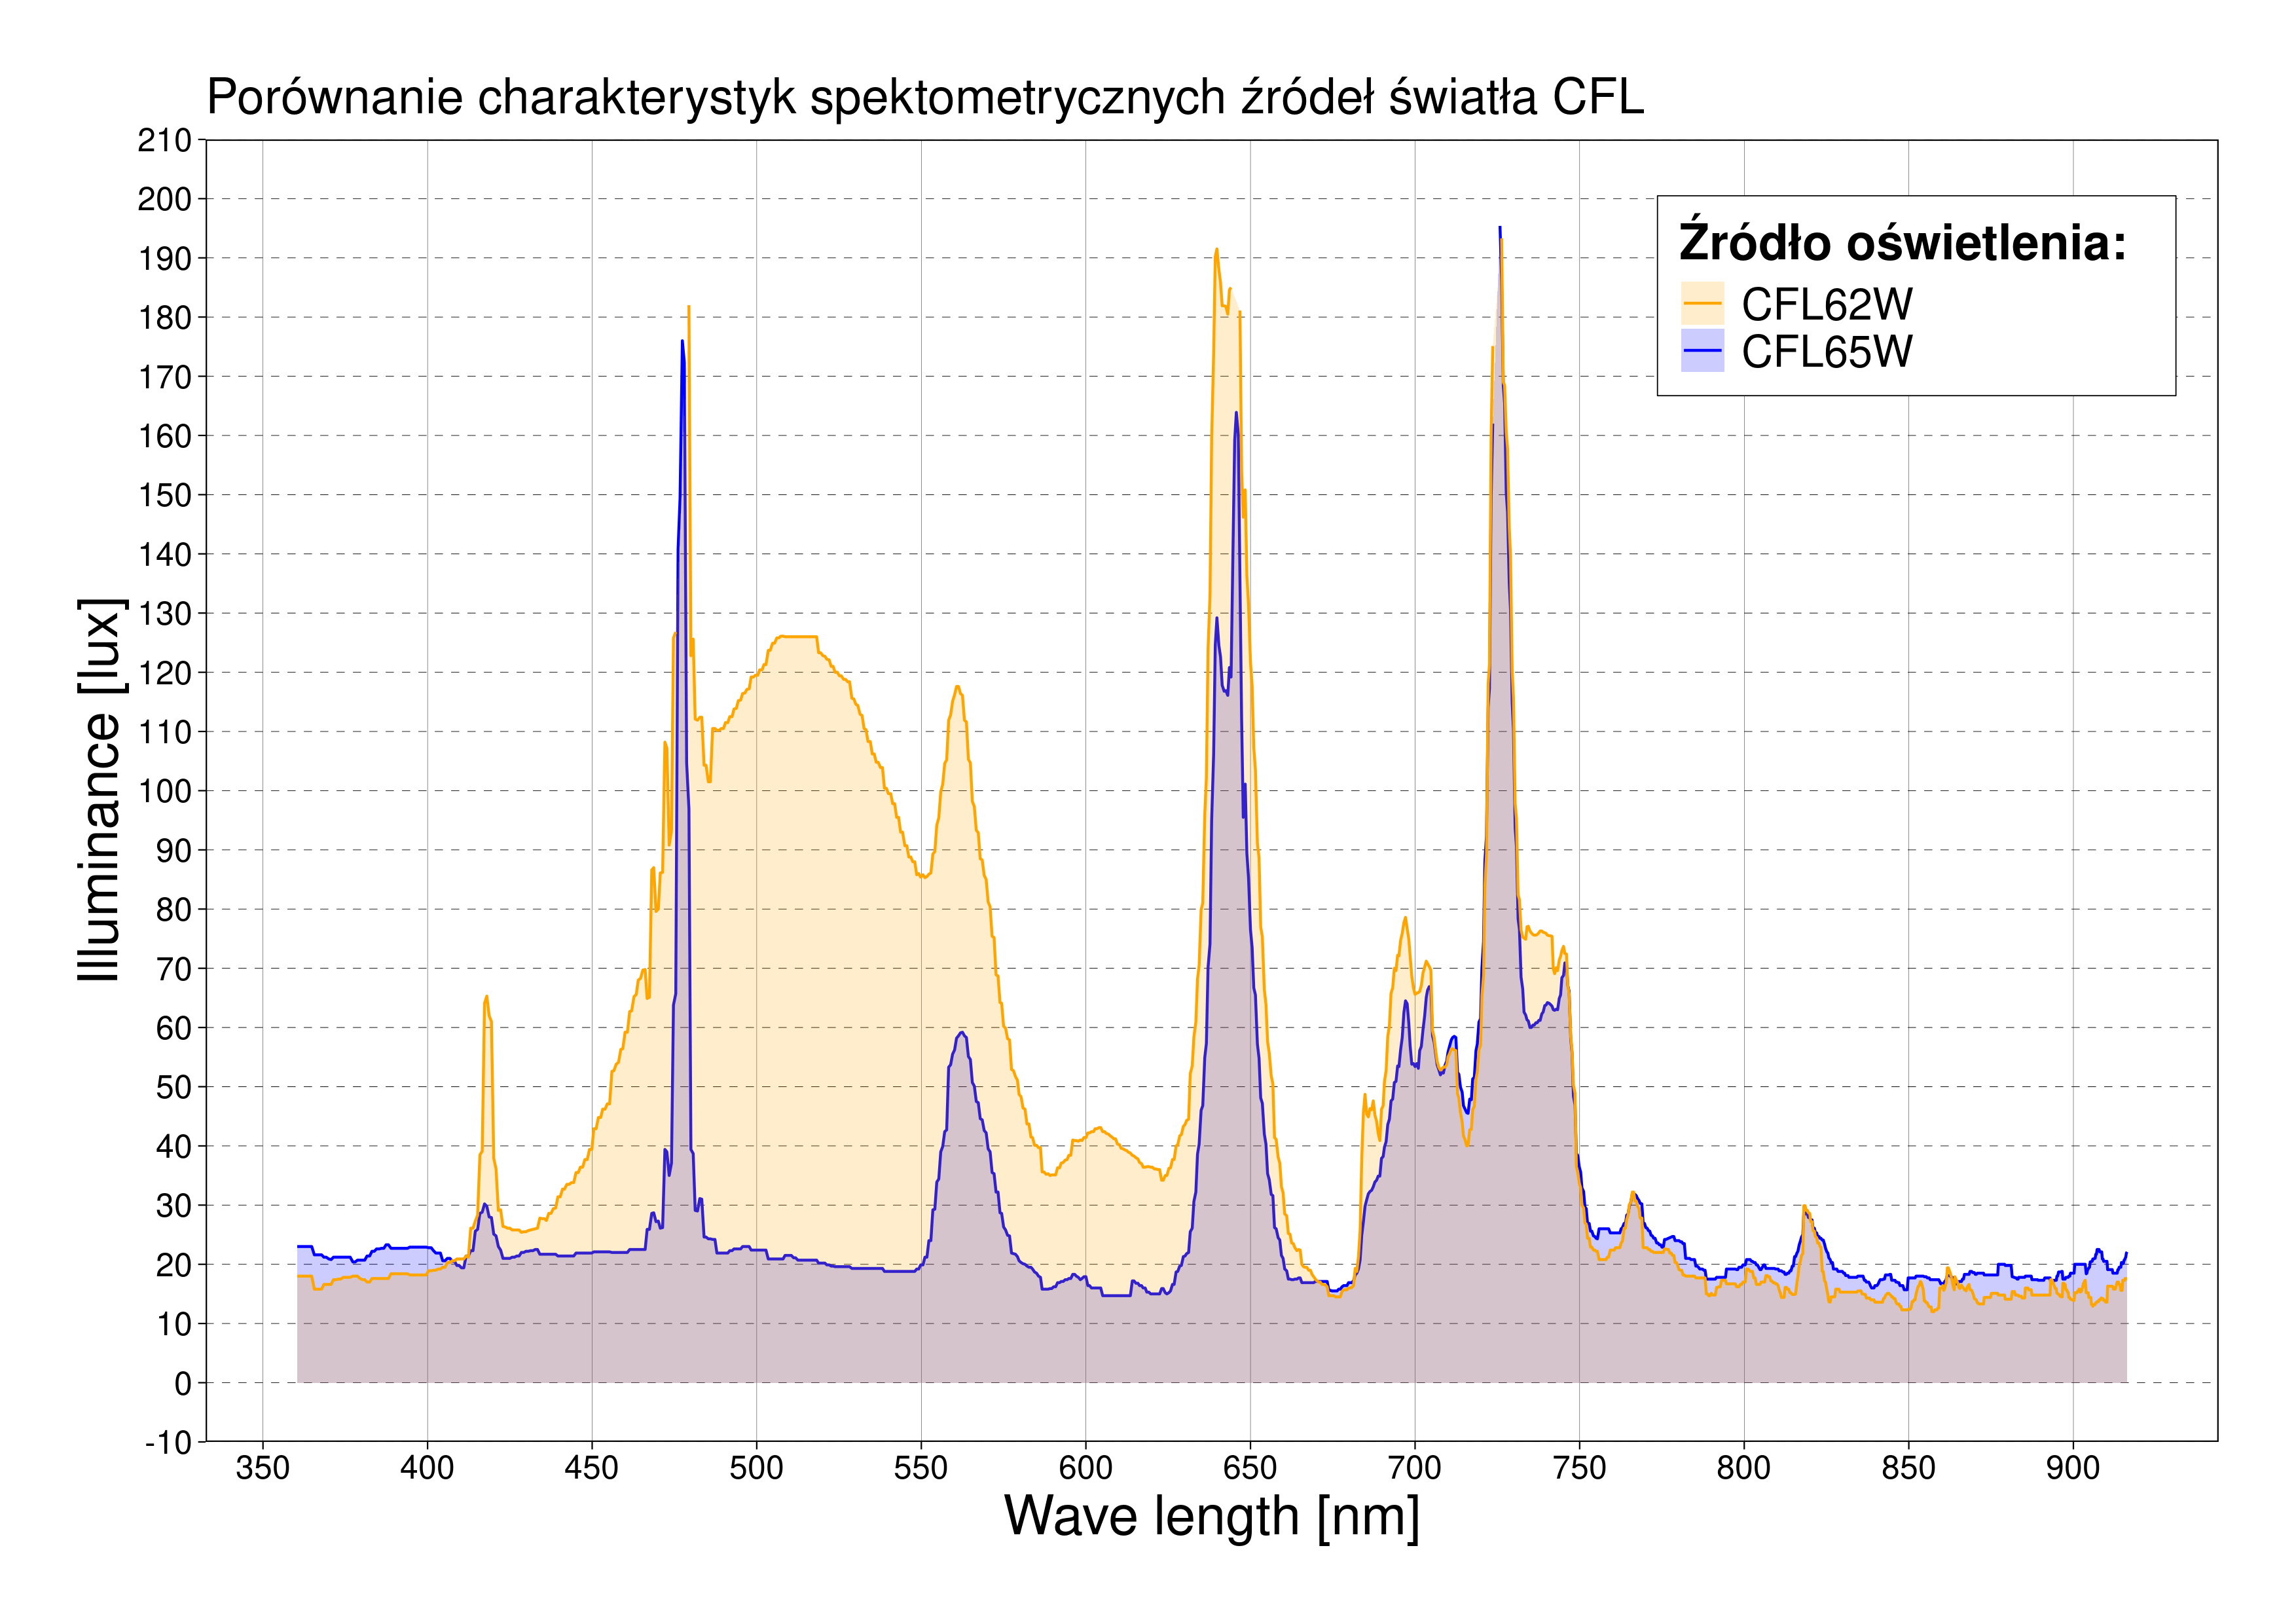
\includegraphics[scale = 0.6]{/home/bork/IdeaProjects/LatexProjects/src/PodstawyTechnikiSensorowej/Lab7/Img/plot4}}
    \justifying Porównując te dwa źródła światła typu CFL możemy zauważyć bardzo dużo podobieńst. Lampa o wyższej mocy posiada
    piki które pokrywają się z lampą o niższej mocy jednak lampa o mocy niższej posiada dodatkowy szeroki pik w zakresie $450-550[nm]$.
    Ta różnica może wynikać z zastosowania dodatkowego luminofora który generuje te długości w przypadku naświetlenia światłem UV.
    Można też zauważyć że źródło o niższej mocy nie posiada niższych amplitud a wręcz przeciwnie można stwierdzić że średnia amplitud
    jest wyższa niż dla lampy mocniejszej. Może to oznaczać że lampa o niższej mocy jest lampą nowej generacji która jest bardziej elektrooszczędna
    gdyż produkując więcej światła posiada mniejsze zużycie energii.
    \subsection{Zastosowanie spektroskopii w chemicznej analizie ilościowej}
    \par Na podstawie pomiarów wyznaczono absorbancję dla kolejnych roztworów oranżu metylowego na podstawie wzoru:
    \begin{gather}
        A=\log_{10}(\frac{I_0}{I})
    \end{gather}
    \par Przykładowo dla najwyższego stężenia oranżu metylowego:
    \begin{gather}
        A=\log_{10}(\frac{167}{158})=\log_{10}(1.056962)=0.0240593
    \end{gather}
    \noident Na podstawie powyższych kalkulacji wykreślono wykres $A=f(C)$ gdzie $C$ stężenie oranżu metylowego:\\
    \noindent\makebox[\textwidth]{
        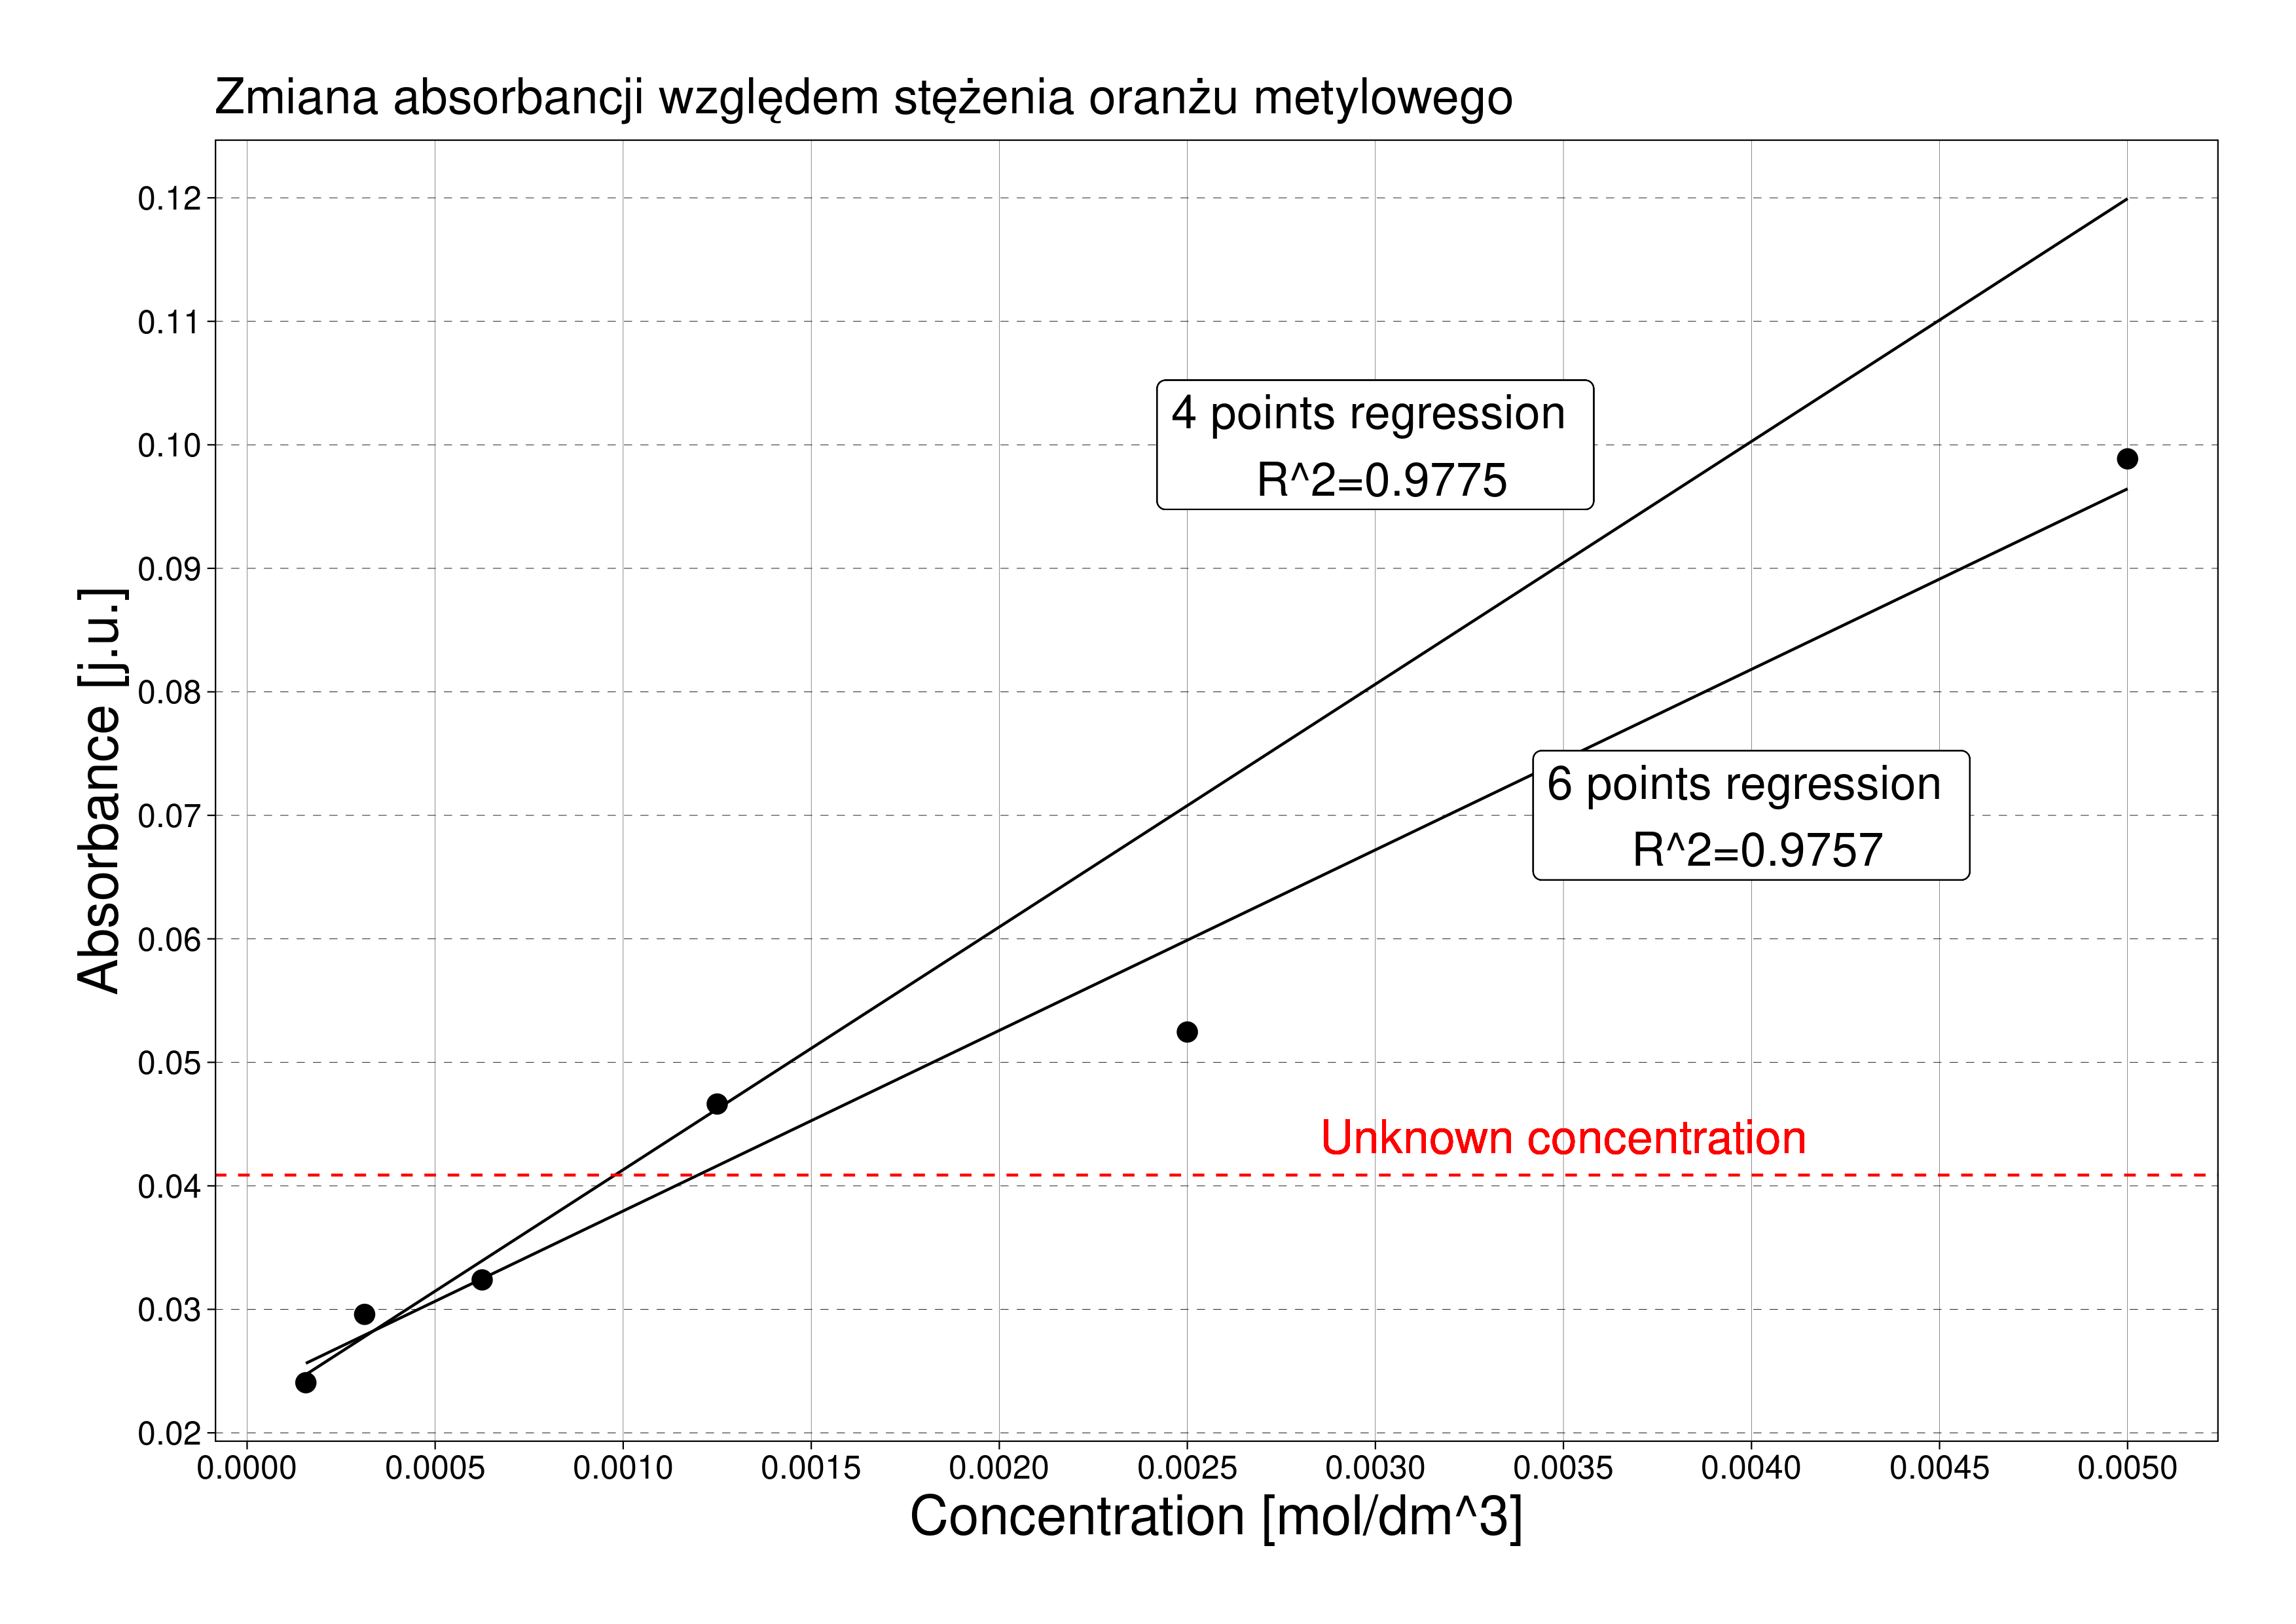
\includegraphics[scale = 0.53]{/home/bork/IdeaProjects/LatexProjects/src/PodstawyTechnikiSensorowej/Lab7/Img/plot2}}
    \indent Na podstawie wykresu wyznaczono dwie krzywe. Jedną aproksymującą pierwsze 4 punkty pomiarowe i drugą aproksysymującą wszystie 6
    punktów. Obie krzywe wykazują dość podobny współczynnik determinacji. Bazując na informacji że liniowość zachodzi dla niższych stężeń
    do obliczeń wybrano krzywą na podstawie pierwszych 4 punktów.\\
    \indent Poniżej przedstawiono wyniki regresji liniowej:
    \begin{gather}
        y=19.6573x+0.0216
    \end{gather}
    \noindent Aby wyznaczyć koncentrację dla butelki X należy przekształcić równanie aby wyznaczało wartość $x$:
    \begin{gather}
        y=19.6573x+0.0216 \\
        y-0.0216=19.6573x \\
        x=\frac{y-0.0216}{19.6573}
    \end{gather}
    \noindent Podstawiając wartość absorbancji dla stężenia X ($A=0.04087288$):
    \begin{gather}
        x=\frac{0.04087288-0.0216}{19.6573}=0.0009804441\left[\frac{mol}{dm^3}\right]\approx 0.001\left[\frac{mol}{dm^3}\right]
    \end{gather}
    \noindent Na podstawie prawa Lamberta-Beera jesteśmy w stanie wyznaczyć molowy współczynnik absorbcji:
    \begin{gather}
        A=\varepsilon lc\\
        \varepsilon=\frac{A}{lc}
    \end{gather}
    \noindent Składnik prawej strony $\frac{A}{c}$ jest niczym innym jak współczynnikiem kierunkowej regresji. Możemy więc
    wyznaczyć molowy współczynnik absorbcji jako (Gdzie $a$ współczynnik kierunkowy regresji):
    \begin{gather}
        \varepsilon=a
    \end{gather}
    \noindent Dla naszych danych:
    \begin{gather}
        \varepsilon=19.6573\left[\frac{dm^3}{mol\ cm}\right]
    \end{gather}

    \subsection{Tabela 1 - wyniki}
    \begin{center}
        \Large\csvreader[tabular = |c|c|c|,
            table head = \hline  \boldmath{$I[lx]$}  & \boldmath{$C[\frac{dm^3}{mol}]$} & \boldmath{$A[j.u.]$}  \\\hline,
            late after line = \\\hline
        ]{Data/outData.csv}{}{
            \csvcolii & \csvcoliii & \csvcoliv
        }
    \end{center}

%    \noindent\makebox[\textwidth]{
%        \includegraphics[scale = 0.7]{/home/bork/IdeaProjects/LatexProjects/src/PodstawyTechnikiSensorowej/Lab6/Img/plot1}}
%    \subsection{Tabela 1}
%    \begin{center}
%        \Large\csvreader[tabular = |c|c|c|c|c|,
%            table head = \hline  \textbf{$x_{gaz}[ppm]$}  & \textbf{$R[k\Omega]$} & \textbf{$I_{max}[\mu A]$}  & \textbf{$G[S]$} & \textbf{$S$}  \\\hline,
%            late after line = \\\hline
%        ]{Data/output.csv}{}{
%            \csvcolii & \csvcoliii & \csvcoliv & \csvcolv  & \csvcolvi
%        }
%    \end{center}
    \section{Wnioski}
    \par Na podstawie pierwszej części ćwiczenia możemy wywnioskować że najprzyjemniejszymi dla oczu źródłami światła będą
    żarótka oraz lampa halogenowa. Jeżeli natomiast potrzebujemy światła które odpowiednio odwzorowuje kolory powierzchni jednocześnie
    mając najlepszą cene względem mocy emisji to naszym wyborem powinna być lampa LED.\\
    \indent Na podstawie drugiej części ćwiczenia mogliśmy zaobserwować zależność wynikającą z prawa Lamberta-Beera oraz nauczyć się
    jak określać stężenie substancji na podstawie jej absorbancji. Na podstawie obliczeń udało się również wyznaczyć stężenie dla
    nieznanej koncentracji oranżu metylowego w butlce "X" równe $0.00098[\frac{mol}{dm^3}]$.



    %Bibliografia
    \vfill
    \footnotesize
    \begin{thebibliography}{3}
        \bibitem{texbook1}
        https://www.researchgate.net/figure/Lighting-efficiency-and-lifetime-of-some-light-sources-10\_tbl1\_283744399
        \bibitem{texbook2}
        https://iarjset.com/upload/2017/april-17/IARJSET\%207.pdf
        \bibitem{texbook3}
        https://en.wikipedia.org/wiki/Spectroscopy
        \bibitem{texbook4}
        https://www.photochemcad.com/databases/common-compounds/azo-dyes/methyl-orange
    \end{thebibliography}
\end{document}
